\documentclass[12pt,reqno,a4paper,oneside]{article}

\usepackage{amsmath,amssymb,amsthm}
\usepackage[english]{babel}
\usepackage[utf8]{inputenc}
\usepackage[T1]{fontenc}

\usepackage{graphicx}

\theoremstyle{plain}
\newtheorem{thm}{Theorem}[section]
\newtheorem{lem}[thm]{Lemma}
\newtheorem{prop}[thm]{Proposition}
\newtheorem{cor}[thm]{Corollary}

\theoremstyle{definition}
\newtheorem*{defn}{Definition}
\newtheorem{exmp}{Example}[section]

\theoremstyle{remark}
\newtheorem*{rem}{Remark}

\begin{document}

\tableofcontents


\section{Introduction}
\label{sec:Introduction}
A problem of lifetime distribution estimation from randomly right-censored observations naturally appears in actuarial and medical statistics as well as in reliability analysis $\#$. In case of independent identically distributed observations \emph{Kaplan-Meier estimator} is usually used $\#$. Consider a model in which each observation is drawn from a finite mixture of distributions. If mixture probabilities (concentrations) vary through the observations, this model is called \emph{mixture model with varying concentrations}. Two modifications of Kaplan-Meier estimator for this model were proposed: the first one by A. Ryzhov $\#$ and the second one by V. Khizanov and R. Maiboroda $\#$. In this paper these two estimators (modifications) are compared via numerical simulations.

The problem statement is considered in Section \ref{sec:Problem_statement}. Section \ref{sec:Simulation_description} is devoted to description of both estimators. Section \ref{sec:Simulation_results} shows results of simulations. Conclusions are presented in Section \ref{sec:Conclusions}.

\section{Problem statement}
\label{sec:Problem_statement}
Let $\mathcal O = \{O_j\}_{j=1}^n$ be a sample from a mixture with varying concentrations. I.e. each $O_j$ belongs to some component $\mathrm{ind}(O_j)\in \{1,\ldots ,M\}$. The true value of $\mathrm{ind}(O_j)$ is not observed. Instead, one is provided with \emph{mixture probabilities}
\begin{equation}
\label{eq:mixture_probabilities}
p_j^m = \mathbb P(\mathrm{ind}(O_j) = m), \, m=1,\ldots, M
\end{equation}
For each subject $O_j$ there exists a positive characteristic $\xi _j = \xi (O_j)$ which is treated as a lifetime. Distribution of each $\xi _j$ depends on the component it belongs to, i.e.:
\begin{equation}
\label{eq:conditional_distribution}
F_m (A) = \mathbb P(\xi _j \in A \mid \mathrm{ind}(O_j) = m), \, m=1,\ldots , M
\end{equation}
\begin{rem}
Mixture probabilities \eqref{eq:mixture_probabilities} satisfy normalization property
\begin{equation}
\label{eq:mix_prob_constraint}
\sum _{m=1}^M p_j^m = 1, \, j = 1,\ldots, n
\end{equation}
\end{rem}

Consider the case in which \emph{true data} $\mathcal D = \{\xi _j\}_{j=1}^n$ are randomly right-censored. That is there exists a sequence of positive random variables $\{c_j\}_{j=1}^n$ such that only \emph{censored data} $\mathcal D^c = \{(\xi _j^*, \delta _j)\}_{j=1}^n$ are observed, where $\xi _j^* = \min (\xi _j, c_j)$ and $\delta _j = \mathbf 1\{\xi _j \leq c_j\}$ for each $j=1,\ldots ,n$. Here, $c_j$'s are called \emph{censors} and their conditional distributions are given by:
\begin{equation}
\label{eq:cens_cond_dist}
G_m (A) = \mathbb P(c _j \in A \mid \mathrm{ind}(O_j) = m),\, m=1,\ldots , M
\end{equation} 

The problem is to estimate conditional distributions $\{F_m\}_{m=1}^M$ from censored data $\mathcal D^c$ and mixture probabilities $\mathbf P = (p_j^m)_{j,m=1}^{n,M}$. Vectors $(\xi _j, c _j)$ are assumed to be independent as well as variables $\xi _j$ and $c_j$ are conditionally independent given $\mathrm{ind}(O_j)$ for each $j=1,\ldots ,n$. Two solutions for this problem are described in subsequent sections. For the sake of simplicity only cumulative distribution functions are considered.

\subsection{Ryzhov estimator}
\label{subsec:ryzhov_estimator}
Suppose a data set $\tilde {\mathcal D}$ is divided into $N$ subsamples $\{\tilde{\mathcal D} _i\}_{i=1}^N$ where each subsample $\tilde{\mathcal D}_i$ comprises i.i.d. random variables $\{\xi _{j} \}_{j=1}^{n_i}$ with the following CDF:
\begin{equation}
\label{eq:Ryzhov_mixture_distribution}
H_i(t) = \sum _{m=1}^M p_i^mF_m(t), \, i = 1,\ldots, N,
\end{equation}
where $p_i^m$ and $F_m$ are defined by \eqref{eq:mixture_probabilities} and \eqref{eq:conditional_distribution} respectively. For each subsample $\tilde{\mathcal{D}}_i$ censors $\{c_j\}_{j=1}^{n_i}$ are i.i.d. with the following CDF:
\begin{equation}
\sum _{m=1}^M p_i^mG_m(t), \, i = 1,\ldots, N,
\end{equation}
where each $G_m, m=1,\ldots, M$ is defined by \eqref{eq:cens_cond_dist}. Thus $\{\xi _{j} \}_{j=1}^{n_i}$ and $\{c_j\}_{j=1}^{n_i}$ together form censored sample $\tilde{\mathcal D}_i^c$.

To estimate conditional distributions $\{F_m\}_{m=1}^M$ in this setting Ryzhov's estimator can be applied $\#$. It is defined in two steps: first one should estimate each $H_i$ by applying Kaplan-Meier estimator to each subsample $\tilde{\mathcal D}^c_i$, and then use these estimations for deriving $\hat F_m$. Suppose that $\{\xi ^* _{j} \}_{j=1}^{n_i}$ in each $\tilde{\mathcal D}_i^c$ are sorted in non-decreasing order as well as each corresponding $\delta_j$ is rearranged following $\xi ^* _j$-th order. Then Ryzhov's estimator takes the form:
\begin{equation}
\hat H^{\mathrm{KM}}_i (t) = 1 - \prod _{j:\xi ^*_{j} \leq t} \Bigg(1 - \frac {\delta _{j}}{n_i - j + 1}\Bigg)
\end{equation}
and
\begin{equation}
\label{eq:ryzhov_estimator}
\hat F^{\mathrm{R}}_m(t) = \sum _{i=1}^N a_i^m \hat H^{\mathrm{KM}}_i(t)
\end{equation}
Here coefficients $a_i^m$ are determined by the $mi$-th element of a matrix
\begin{equation}
(\mathbf P^\top \boldsymbol{\Sigma}^{-1}\mathbf P)^{-1} \mathbf P^\top \boldsymbol{\Sigma}^{-1},
\end{equation}
where $\mathbf P = (p_i^m)_{i,m=1}^{N,M}$ is a mixture probability matrix and matrix $\boldsymbol{\Sigma} = \mathbf{diag}(\sigma ^2 _1(t), \ldots, \sigma ^2 _N(t))$ is a diagonal matrix which contains variances of Kaplan-Meier estimator, i.e. $\sigma ^2_i(t) = \mathbb V [\hat H^{\mathrm{KM}}_i(t)], i=1,\ldots, N$. Since each $\sigma ^2_i(t)$ depends on unknown distributions $H_1(t), \ldots, H_N(t)$ one can use Greenwood's formula in order to estimate it:
\begin{equation}
\hat \sigma ^2_i (t) = (1 - \hat H^{\mathrm{KM}}_i(t))^2 \sum _{j:\xi _{j} \leq t}\frac {\delta _{j}}{(n_i - j)(n_i - j + 1)}
\end{equation}
\begin{thm}[Ryzhov]
Suppose all $n_i = O(n)$, where $n = n_1 + \ldots + n_N$ and mixture probability matrix $\mathbf P$ has full rank. Then $\hat F^R_m$ defined by \eqref{eq:ryzhov_estimator} is uniformly consistent and asymptotically normal estimator of $F_m$ for each $m=1,\ldots , M$.
\end{thm}


\subsection{Product-integral estimator}
Unlike Ryzhov's estimator an estimator proposed by V. Khizanov and R. Maiboroda $\#$ does not require dividing censored data into subsamples. Suppose for simplicity that $\{\xi ^* _j\}_{j=1}^n$ are ordered in non-decreasing order as well as each corresponding $\delta_j$ is permutated with respect to $\xi ^*_j$. Then the product-integral estimator takes the form:
\begin{equation}
\label{eq:khizanov_maiboroda_estimator}
\hat F^{\mathrm{PI}}_m(t) = 1 - \prod _{j : \xi ^*_j \leq t}\bigg( 1 - \frac {a_j^m \delta _j}{1 - \sum _{i:\xi ^*_i < t} a_i^m} \bigg)
\end{equation}
where coefficients $a_j^m$ are equal to $mj$-th element of a matrix
\begin{equation}
(\mathbf P^\top \mathbf P)^{-1}\mathbf P^\top
\end{equation}
with a mixture probability matrix $\mathbf P=(p_{j}^m)_{j,m=1}^{n, M}$.
\begin{thm}
Let mixture probability matrix $\mathbf P$ satisfy the following property: 
\begin{equation*}
\sqrt{\frac{\ln n}{n}}(\det (\mathbf P^\top \mathbf P))^{-3} \to 0, n \to \infty
\end{equation*}
Then $\hat F^{\mathrm{PI}}_m$ defined by \eqref{eq:khizanov_maiboroda_estimator} is uniformly consistent estimator of $F_m$ for each $m=1,\ldots, M$.
\end{thm}
\begin{rem}
Asymptotic normality of Khizanov-Maiboroda's estomator has not been proven yet.
\end{rem}



\section{Simulation description}
\label{sec:Simulation_description}
This section introduces settings for comparison of two estimators described previously. For each experiment the mixture probability matrix $\mathbf P$ is generated randomly using the following procedure:
\begin{itemize}
	\item[1.] sample $n M$ independent random variables from $\mathcal U(0, 1)$, which form an $n\times M$ matrix $\mathbf A$
	\item[2.] divide each row of $\mathbf A$ by the sum of elements in that row
	\item[3.] if $\det (\mathbf A ^\top \mathbf A) > 0.2$ set $\mathbf P = \mathbf A$, otherwise go to step 1
\end{itemize}
\begin{rem}
The last step in previous algorithm is performed in order to avoid ill-conditioned cases.
\end{rem}
Since Ryzhov's estimator requires special form of input data, the following procedure to the mixture probability matrix $\mathbf P$ is applied : 
\begin{itemize}
	\item[1.] Fix a number of bins $N\geq 2$ and consider a partition $\{\mathcal B_1, \ldots, \mathcal B_N\}$ of unit interval $[0, 1)$: $$ \bigcup _{i = 1}^N \mathcal B_i = \bigcup _{i = 1}^N[\frac {i - 1}{N}, \frac iN)$$
	\item[2.] Assign each $p_j^m$ to the center of a bin it belongs to
\end{itemize}
\begin{rem}
A subsample of censored data $\mathcal D^c$ which corresponding mixture probabilities belong to the $i$-th bin forms $\tilde{\mathcal D}_i^c$.
\end{rem}
Next section provides simulation results for two-component mixture, i.e. $M=2$, where the quantity
\begin{equation}
\mathbb E \sup _{t} |\hat F_m(t) - F_m(t)|, \, m=1,2
\end{equation}
is of interest.

\section{Simulation results}
\label{sec:Simulation_results}
Let $F_1\sim \chi ^2_1$ and $F_2\sim \chi ^2_2$ have chi-squared distribution with $1$ and $2$ degrees of freedom respectively. All censors $c_j$ have the same uniform distribution $G\sim \mathcal U(0, 8)$ which corresponds to approximately $20\%$ of censored observations. 

Figure \ref{fig:1} provides simulation results for different number of bins $N$. An $X$ axis represents a sample size $n$ while $Y$ axis represents an estimation for the quantity $\mathbb E \sup _{t} |\hat F_m(t) - F_m(t)|$ based on 1000 independent experiments.

As one can see, for sufficiently large sample size and reasonable number of bins estimators performs almost equally. The amount of bins can be treated as a bias-variance trade-off, i.e. small values of $N$ produces high bias low variance estimations and vice versa.


\section{Conclusions}
\label{sec:Conclusions}
Following simulation results product-integral estimator generally outperforms one proposed by Ryzhov, but for large samples this advantage may be negligible. However, for small size samples  Ryzhov's estimator remains still reasonable and can provide better estimations in some cases.


\begin{figure}
\centering
\caption{\label{fig:1}Error comparison for different number of bins $N$}
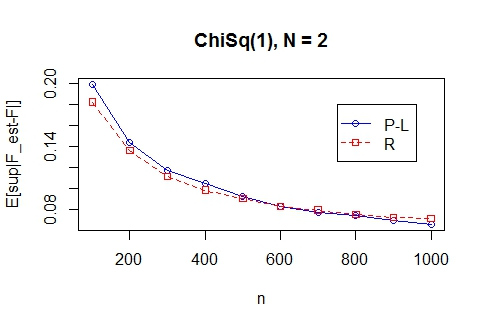
\includegraphics[scale=0.35]{12.jpeg}
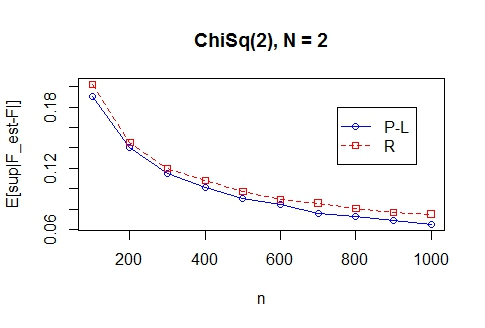
\includegraphics[scale=0.35]{22.jpeg}
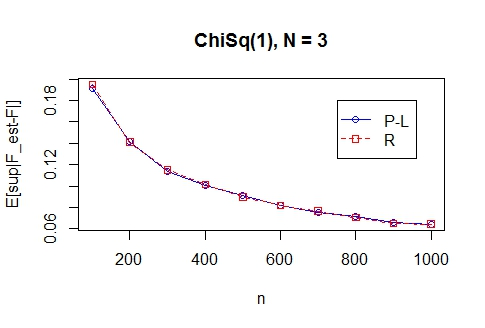
\includegraphics[scale=0.35]{13.jpeg}
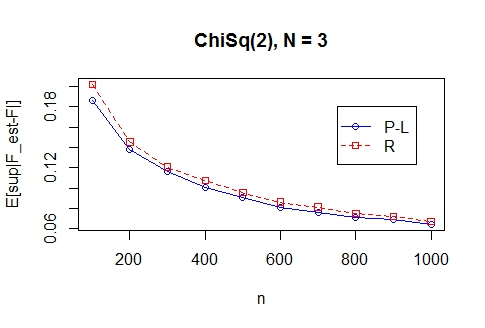
\includegraphics[scale=0.35]{23.jpeg}
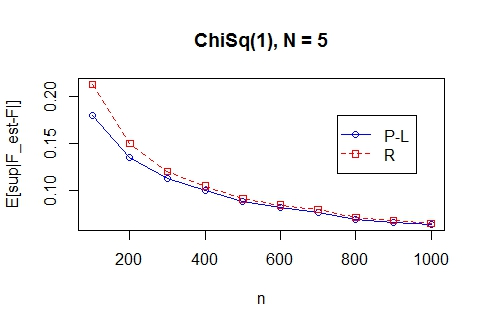
\includegraphics[scale=0.35]{15.jpeg}
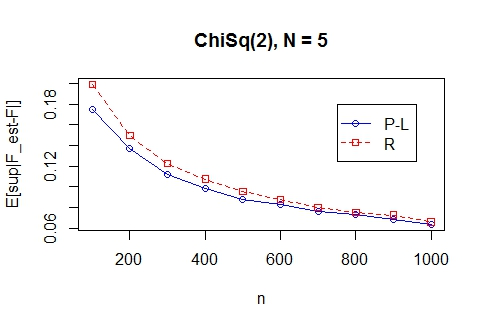
\includegraphics[scale=0.35]{25.jpeg}
\end{figure}

\end{document}
